\documentclass[journal,12pt,twocolumn]{IEEEtran}
\usepackage[none]{hyphenat}
\usepackage{graphicx}
\usepackage{listings}
\usepackage[english]{babel}
\usepackage{graphicx}
\usepackage{caption} 
\usepackage{amsmath}
\usepackage{hyperref}
\usepackage{amsmath,amsfonts,amssymb}
\usepackage{booktabs}
\usepackage{array}
\let\vec\mathbf

\title{\textbf{\\Circle Assignment}}
\author{Sinkona Chinthamalla - FWC22054}

\newcommand{\myvec}[1]{\ensuremath{\begin{pmatrix}#1\end{pmatrix}}}
\newcommand{\mydet}[1]{\ensuremath{\begin{vmatrix}#1\end{vmatrix}}}
\providecommand{\brak}[1]{\ensuremath{\left(#1\right)}}
\providecommand{\lbrak}[1]{\ensuremath{\left(#1\right.}}
\providecommand{\rbrak}[1]{\ensuremath{\left.#1\right)}}
\providecommand{\sbrak}[1]{\ensuremath{{}\left[#1\right]}}

\begin{document}
\maketitle

\section{Question}
\textbf{\textit{Chapter 8, Section-B, Q(21):} The circle \\ $ x^2+y^2= 4x+8y+5 $ intersects the line $ 3x-4y = m $ at two distinct points if}

\begin{figure}[h!]
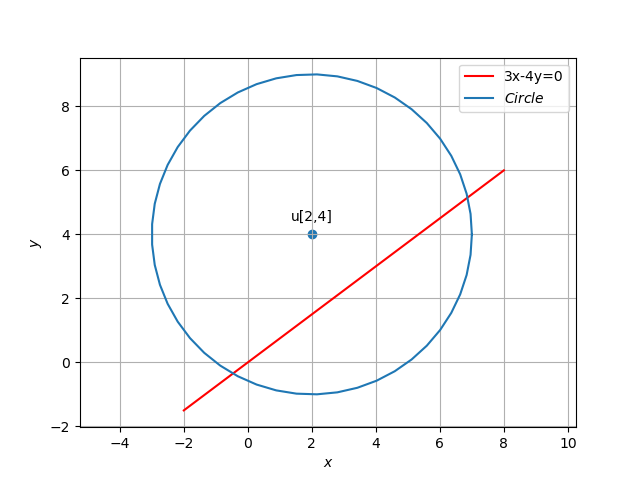
\includegraphics[scale=0.55]{c.png}
\caption{Circle with the line intersecting at two distinct points}
\end{figure}

\section{Construction}
\centering
\vspace{0.2cm}
{
\setlength\extrarowheight{2pt}
\begin{tabular}{|c|c|c|}
	\hline
	\textbf{Symbol}&\textbf{Value}&\textbf{Description}\\
	\hline
	\textbf{O} & 
	$\begin{pmatrix}
     2 \\
     4
    \end{pmatrix}$ & Center of Circle \\
	\hline
	r & 5 & Radius of Circle\\
	\hline
	\textbf{n} & 
	$ \begin{pmatrix}
      3 \\
     -4
    \end{pmatrix}$ & Normal vector\\
	\hline
	$ \vec{P_1}$ & $\begin{pmatrix}
     5 \\
     0
    \end{pmatrix}$ & Point of Contact P1 \\
	\hline
	$ \vec{P_2}$ & $\begin{pmatrix}
     -1 \\
      8
    \end{pmatrix}$ & Point of Contact P2 \\
	\hline
\end{tabular}
}

\section{Solution}
\raggedright The equation of a conic with directrix $\vec{n}^\intercal\vec{x} = c$, eccentricity e and focus \textbf{F} is given by
\begin{align}
\vec{x}^{\top}\vec{V}\vec{x}+2\vec{u}^{\top}\vec{x}+f = 0 
\end{align}
where
\begin{align}
\vec{V} = \begin{pmatrix}
1 & 0\\
0 & 1
\end{pmatrix} \\
\vec{u} = \begin{pmatrix}
     -2 \\
     -4
    \end{pmatrix}  \\
f = -5  
\end{align}

If $\vec{V}^{-1}$ exists, given the normal vector $\vec{n}$, the tangent points of contact to $\vec{n}^\intercal\vec{x} = c$ are given by
\begin{align}
\vec{q}_i &= \vec{V}^{-1}\brak{\kappa_i \vec{n}-\vec{u}}, i = 1,2
\\
\text{where }\kappa_i &= \pm \sqrt{
\frac{
f_0
}
{
\vec{n}^{\top}\vec{V}^{-1}\vec{n}
}
}
\end{align}
\begin{equation}
f_0=\vec{u^\top} \vec{V^{-1}} \vec{u}-f
\end{equation}
Given equation of line,
\begin{align}
3x-4y=m \\
\begin{pmatrix}
3 & -4
\end{pmatrix}
\vec{x} = m  
\end{align}

Substituting (2), (3), (4) and (9) in (6) yields
\begin{align}
\kappa = \pm 1
\end{align}

By substituting (10) in (5), we get points of contact $\vec{P_1}$ and $\vec{P_2}$\\
$\text{For} \quad \kappa = 1 $
%\begin{equation}
%\vec{q} = \begin{bmatrix}
%                 1 & 0\\
%                 0 & 1
%          \end{bmatrix} 
%\biggr[\begin{pmatrix}
%      3 \\
%     -4
%    \end{pmatrix} - \begin{pmatrix}
%                    -2 \\
%                    -4
%                    \end{pmatrix} \biggr]
%\end{equation}
\begin{align}
\vec{P_1} = \begin{pmatrix}
      5 \\
      0
    \end{pmatrix}
    \label{eq-1}
\end{align}
$ \text{For} \quad \kappa = -1 $
\begin{align}
\vec{P_2} = \begin{pmatrix}
     -1  \\
      8
    \end{pmatrix}
\label{eq-2}
\end{align}

Substituiting $\vec{P_1}$ and $\vec{P_2}$ in (9) yields
\begin{align}
\begin{pmatrix}
3 & -4
\end{pmatrix}
\begin{pmatrix}
      5 \\
      0
    \end{pmatrix} = m_1  \\
m_1 = 15    \\
\begin{pmatrix}
3 & -4
\end{pmatrix}
\begin{pmatrix}
      -1 \\
       8
    \end{pmatrix} = m_2  \\
m_2 = -35    
\end{align}

Therefore, the range of m is\\
\vspace{0.2cm}
\centering 
$-35 < m < 15$

\begin{figure}[h!]
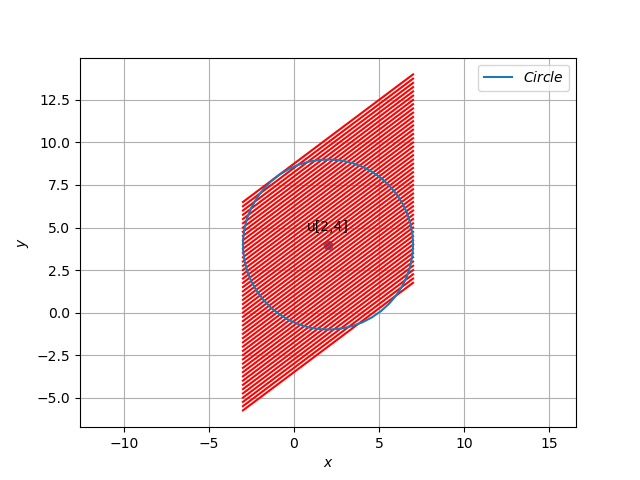
\includegraphics[scale=0.55]{cr.png}
\caption{Circle with the line 3x-4y=m}
\end{figure}

\newpage
Get the python code from
\begin{table}[h]
\large
\centering
\begin{tabular}{|l|}
\hline
https://github.com/SinkonaChinthamalla/fwc/
\\blob/main/matrix/line/codes \\
\hline
\end{tabular}
\end{table}	
\end{document}